\RequirePackage[T1]{fontenc}            
\RequirePackage[utf8]{inputenc}         
\RequirePackage{filecontents}

\newcommand{\myName}{Alessandro Zangari}
\newcommand{\myTitle}{DataMole User Manual}           
\newcommand{\myUni}{Università degli Studi di Padova}    
\newcommand{\myFaculty}{Corso di Laurea Magistrale in Informatica}

\begin{filecontents*}{\jobname.xmpdata}
	\Title{\myTitle}
	\Author{\textcopyright\ \myName,\ \myUni,\ \myFaculty}
	\Subject{User manual for DataMole}
	\Keywords{Preprocessing tool\sep DataMole\sep User manual}
	\Language{en-GB}
	\Copyright{Copyright \copyright\ 2020,\ \myName,\ \myUni,\ \myFaculty}
	\Date{2020-10-02}
\end{filecontents*}

\author{\myName}
\title{\myTitle}

\documentclass[10pt,   
               a4paper,                 
%               twoside,                 
%               openright,           
               english,                 
               ]{article}    

%**************************************************************
% Importazione package
%************************************************************** 

\usepackage{colorprofiles}
%\usepackage{amsmath,amssymb,amsthm}
\usepackage[table, rgb]{xcolor}

\usepackage[english]{babel}

%\usepackage{caption}                   

%\usepackage{dirtree}

\usepackage{csquotes}                   

\usepackage{graphicx}      

%\usepackage{nameref} 
%\usepackage[english]{varioref}

\usepackage{setspace}

\usepackage{titlesec}

\usepackage[a-2u]{pdfx}[2018/12/22]

%Workaround for missing metadata for keywords
\makeatletter
\def\sep{, }
%\pdfx@topdfstring\pdfx@Author\xmp@Author
\pdfx@topdfstring\pdfx@pdfKeywords\xmp@Keywords
\makeatother

\usepackage[binding=5mm]{layaureo}

\usepackage{listings}

\usepackage{multirow}

\usepackage[backend=biber,style=numeric-comp,hyperref,backref]{biblatex}

%\usepackage{pxfonts}
%\usepackage{newpxtext}
%\usepackage{newpxmath}
\usepackage[capitalise]{cleveref}

%**************************************************************
% file contenente le impostazioni della tesi
%**************************************************************

%**************************************************************
% Impostazioni di impaginazione
% see: http://wwwcdf.pd.infn.it/AppuntiLinux/a2547.htm
%**************************************************************

\setlength{\parindent}{0pt}   % larghezza rientro della prima riga
\setlength{\parskip}{0pt}   % distanza tra i paragrafi


%**************************************************************
% Impostazioni di biblatex
%**************************************************************
\bibliography{bibliography} % database di biblatex 

%\defbibheading{bibliography} {
%    \cleardoublepage
%    \phantomsection
%    \addcontentsline{toc}{chapter}{\bibname}
%    \chapter*{\bibname\markboth{\bibname}{\bibname}}
%}

\setlength\bibitemsep{1.5\itemsep} % spazio tra entry

%\DeclareBibliographyCategory{opere}
%\DeclareBibliographyCategory{web}

%**************************************************************
% Impostazioni di caption
%**************************************************************
%\captionsetup{
%    tableposition=top,
%    figureposition=bottom,
%    font=small,
%    format=hang,
%    labelfont=bf
%}

%**************************************************************
% Impostazioni di glossaries
%**************************************************************
%\input{special_sections/glossary} % database di termini
%\makeglossaries


%**************************************************************
% Impostazioni di graphicx
%**************************************************************

%\setcounter{secnumdepth}{3}

\setcounter{secnumdepth}{4}

\titleformat{\paragraph} {\normalfont\normalsize\bfseries}{\theparagraph}{1em}{}
\titlespacing*{\paragraph} {0pt}{3.25ex plus 1ex minus .2ex}{1.5ex plus .2ex}

%\newcommand{\lineparagraph}[1]{\paragraph{#1}\mbox{}\\}
\newcommand{\lineparagraph}[1]{\paragraph{#1}}

% TABELLE STRETCH
%\renewcommand{\arraystretch}{1.5}
%\setlength{\arrayrulewidth}{1.2pt}


% table colors

\definecolor{myblue}{rgb}{0.0, 0.47, 0.75}
\definecolor{mylightgray}{RGB}{242, 242, 242}
\definecolor{OliveGreen}{rgb}{0.55, 0.71, 0.0}
%\definecolor{tableCol}{rgb}{0.88,1,1}
\colorlet{tableCol}{mylightgray}
%\definecolor{tableHead}{HTML}{EFEFEF}
\colorlet{tableHead}{myblue}


%**************************************************************
% Impostazioni di hyperref
%**************************************************************
\hypersetup{
    %hyperfootnotes=false,
    %pdfpagelabels,
    %draft,	% = elimina tutti i link (utile per stampe in bianco e nero)
    colorlinks=true,
    linktocpage=true,
    pdfstartpage=1,
    pdfstartview=,
    % decommenta la riga seguente per avere link in nero (per esempio per la stampa in bianco e nero)
    %colorlinks=false, linktocpage=false, pdfborder={0 0 0}, pdfstartpage=1, pdfstartview=FitV,
    breaklinks=true,
    pdfpagemode=UseNone,
    pageanchor=true,
    pdfpagemode=UseOutlines,
    plainpages=false,
    bookmarksnumbered,
    bookmarksopen=true,
    bookmarksopenlevel=1,
    hypertexnames=true,
    pdfhighlight=/O,
    %nesting=true,
    %frenchlinks,
    urlcolor=webbrown,
    linkcolor=myblue,
    citecolor=webgreen
}


%\makeatletter
%%Create an OutputIntent in order to correctly specify colours
%\immediate\pdfobj stream attr{/N 3} file{AdobeRGB1998.icc}
%\edef\iccobj{\the\pdflastobj}
%\pdfcatalog{%
%/OutputIntents [
%<<
%/Type /OutputIntent
%/S/GTS_PDFA1
%/DestOutputProfile \iccobj\space 0 R
%/OutputConditionIdentifier (AdobeRGB1998)
%/Info (AdobeRGB1998)
%>>
%]
%}
%\makeatother

%**************************************************************
% Impostazioni di itemize
%**************************************************************
%\renewcommand{\labelitemi}{$\ast$}

%\renewcommand{\labelitemi}{$\bullet$}
%\renewcommand{\labelitemii}{$\cdot$}
%\renewcommand{\labelitemiii}{$\diamond$}
%\renewcommand{\labelitemiv}{$\ast$}


%**************************************************************
% Impostazioni di listings
%**************************************************************
\lstset{
    language=[LaTeX]Tex,%C++,
    keywordstyle=\color{RoyalBlue}, %\bfseries,
    basicstyle=\small\ttfamily,
    %identifierstyle=\color{NavyBlue},
    commentstyle=\color{Green}\ttfamily,
    stringstyle=\rmfamily,
    numbers=none, %left,%
    numberstyle=\scriptsize, %\tiny
    stepnumber=5,
    numbersep=8pt,
    showstringspaces=false,
    breaklines=true,
    frameround=ftff,
    frame=single
}

\lstdefinelanguage{JavaScript}{
    keywords={typeof, new, true, false, catch, function, return, null, catch, switch, var, if, in, while, do, else, case, break},
    keywordstyle=\color{blue}\bfseries,
    ndkeywords={class, export, boolean, throw, implements, import, this},
    ndkeywordstyle=\color{gray}\bfseries,
    identifierstyle=\color{black},
    sensitive=false,
    comment=[l]{//},
    morecomment=[s]{/*}{*/},
    commentstyle=\color{purple}\ttfamily,
    stringstyle=\color{red}\ttfamily,
    morestring=[b]',
    morestring=[b]"
}

\lstset{
    language=JavaScript,
    backgroundcolor=\color{lightgray},
    extendedchars=true,
    basicstyle=\footnotesize\ttfamily,
    showstringspaces=false,
    showspaces=false,
    numbers=left,
    numberstyle=\footnotesize,
    numbersep=9pt,
    tabsize=2,
    frame=single,
    breaklines=true,
    showtabs=false,
    captionpos=b
}
%
%%**************************************************************
%% Impostazioni di xcolor
%%**************************************************************
\definecolor{webgreen}{rgb}{0,.5,0}
\definecolor{webbrown}{rgb}{.6,0,0}


%**************************************************************
% Altro
%**************************************************************

%\newcommand{\omissis}{[\dots\negthinspace]} % produce [...]
%
%% eccezioni all'algoritmo di sillabazione
%\hyphenation
%{
%    ma-cro-istru-zio-ne
%    gi-ral-din
%}
%
%%\newcommand{\sectionname}{sezione}
%%\addto\captionsitalian{\renewcommand{\figurename}{Figura}
%%    \renewcommand{\tablename}{Tabella}}
%
%
%\newcommand{\glsfirstoccur}{\ap{{[g]}}}
%
\newcommand{\intro}[1]{\emph{\textsf{#1}}}

%**************************************************************
% Environment per ``rischi''
%**************************************************************
%\newcounter{riskcounter}                % define a counter
%\setcounter{riskcounter}{0}             % set the counter to some initial value
%
%%%%% Parameters
%% #1: Title
%\newenvironment{risk}[1]{
%    \refstepcounter{riskcounter}        % increment counter
%    \par \noindent                      % start new paragraph
%    \textbf{\arabic{riskcounter}. #1}   % display the title before the 
%    % content of the environment is displayed 
%}{
%    \par\medskip
%}
%
%\newcommand{\riskname}{Rischio}
%
%\newcommand{\riskdescription}[1]{\textbf{\\Descrizione:} #1.}
%
%\newcommand{\risksolution}[1]{\textbf{\\Soluzione:} #1.}
%
%%**************************************************************
%% Environment per ``use case''
%%**************************************************************
%\newcounter{usecasecounter}             % define a counter
%\setcounter{usecasecounter}{0}          % set the counter to some initial value
%
%%%%% Parameters
%% #1: ID
%% #2: Nome
%\newenvironment{usecase}[2]{
%    \renewcommand{\theusecasecounter}{\usecasename #1}  % this is where the display of 
%    % the counter is overwritten/modified
%    \refstepcounter{usecasecounter}             % increment counter
%    \vspace{10pt}
%    \begin{mdframed}[style=uc]
%        \par \noindent		                        % start new paragraph
%        {\large \textbf{\usecasename #1: #2}}       % display the title before the 
%        % content of the environment is displayed 
%        \medskip
%        }{
%        \medskip
%    \end{mdframed}
%}
%
%
%\newcommand{\usecasename}{UC-}
%
%\newcommand{\usecaseactors}[1]{\textbf{\\Attori Principali:} #1. \vspace{4pt}}
%\newcommand{\usecasepre}[1]{\textbf{\\Precondizioni:} #1. \vspace{4pt}}
%\newcommand{\usecasedesc}[1]{\textbf{\\Descrizione:} #1. \vspace{4pt}}
%\newcommand{\usecasepost}[1]{\textbf{\\Postcondizioni:} #1. \vspace{4pt}}
%\newcommand{\usecasealt}[1]{\textbf{\\Scenari Alternativi:} #1. \vspace{4pt}}

%**************************************************************
% Environment per ``namespace description''
%**************************************************************

%\newenvironment{namespacedesc}{
%    \vspace{10pt}
%    \par \noindent                              % start new paragraph
%    \begin{description}
%        }{
%    \end{description}
%    \medskip
%}
%
%\newcommand{\classdesc}[2]{\item[\textbf{#1:}] #2}


%**************************************************************
% Colori per shaded (blocchi di codice)
%**************************************************************


%\newcommand{\VerbBar}{|}
%\newcommand{\VERB}{\Verb[commandchars=\\\{\}]}
%\DefineVerbatimEnvironment{Highlighting}{Verbatim}{commandchars=\\\{\}}
%% Add ',fontsize=\small' for more characters per line
%\newenvironment{Shaded}{}{}
%\newcommand{\AlertTok}[1]{\textcolor[rgb]{1.00,0.00,0.00}{\textbf{#1}}}
%\newcommand{\AnnotationTok}[1]{\textcolor[rgb]{0.38,0.63,0.69}{\textbf{\textit{#1}}}}
%\newcommand{\AttributeTok}[1]{\textcolor[rgb]{0.49,0.56,0.16}{#1}}
%\newcommand{\BaseNTok}[1]{\textcolor[rgb]{0.25,0.63,0.44}{#1}}
%\newcommand{\BuiltInTok}[1]{#1}
%\newcommand{\CharTok}[1]{\textcolor[rgb]{0.25,0.44,0.63}{#1}}
%\newcommand{\CommentTok}[1]{\textcolor[rgb]{0.38,0.63,0.69}{\textit{#1}}}
%\newcommand{\CommentVarTok}[1]{\textcolor[rgb]{0.38,0.63,0.69}{\textbf{\textit{#1}}}}
%\newcommand{\ConstantTok}[1]{\textcolor[rgb]{0.53,0.00,0.00}{#1}}
%\newcommand{\ControlFlowTok}[1]{\textcolor[rgb]{0.00,0.44,0.13}{\textbf{#1}}}
%\newcommand{\DataTypeTok}[1]{\textcolor[rgb]{0.56,0.13,0.00}{#1}}
%\newcommand{\DecValTok}[1]{\textcolor[rgb]{0.25,0.63,0.44}{#1}}
%\newcommand{\DocumentationTok}[1]{\textcolor[rgb]{0.73,0.13,0.13}{\textit{#1}}}
%\newcommand{\ErrorTok}[1]{\textcolor[rgb]{1.00,0.00,0.00}{\textbf{#1}}}
%\newcommand{\ExtensionTok}[1]{#1}
%\newcommand{\FloatTok}[1]{\textcolor[rgb]{0.25,0.63,0.44}{#1}}
%\newcommand{\FunctionTok}[1]{\textcolor[rgb]{0.02,0.16,0.49}{#1}}
%\newcommand{\ImportTok}[1]{#1}
%\newcommand{\InformationTok}[1]{\textcolor[rgb]{0.38,0.63,0.69}{\textbf{\textit{#1}}}}
%\newcommand{\KeywordTok}[1]{\textcolor[rgb]{0.00,0.44,0.13}{\textbf{#1}}}
%\newcommand{\NormalTok}[1]{#1}
%\newcommand{\OperatorTok}[1]{\textcolor[rgb]{0.40,0.40,0.40}{#1}}
%\newcommand{\OtherTok}[1]{\textcolor[rgb]{0.00,0.44,0.13}{#1}}
%\newcommand{\PreprocessorTok}[1]{\textcolor[rgb]{0.74,0.48,0.00}{#1}}
%\newcommand{\RegionMarkerTok}[1]{#1}
%\newcommand{\SpecialCharTok}[1]{\textcolor[rgb]{0.25,0.44,0.63}{#1}}
%\newcommand{\SpecialStringTok}[1]{\textcolor[rgb]{0.73,0.40,0.53}{#1}}
%\newcommand{\StringTok}[1]{\textcolor[rgb]{0.25,0.44,0.63}{#1}}
%\newcommand{\VariableTok}[1]{\textcolor[rgb]{0.10,0.09,0.49}{#1}}
%\newcommand{\VerbatimStringTok}[1]{\textcolor[rgb]{0.25,0.44,0.63}{#1}}
%\newcommand{\WarningTok}[1]{\textcolor[rgb]{0.38,0.63,0.69}{\textbf{\textit{#1}}}}
%
%% mdframed properties
%
%%\mdfsetup{% specificare proprietà di mdframed
%
%%}
%
%\mdfdefinestyle{code}{%
%    middlelinewidth=0.3pt,
%    roundcorner=5pt,
%    innertopmargin=0.2cm,
%    innerbottommargin=0.2cm,
%    nobreak=true}
%
%\mdfdefinestyle{folder}{%
%    middlelinewidth=0.3pt,
%    roundcorner=5pt}
%
%\mdfdefinestyle{uc}{%
%    middlelinewidth=0.3pt,
%    innertopmargin=0.3cm,
%    innerbottommargin=0.1cm,
%    skipabove=0cm,
%    skipbelow=0cm,
%    nobreak=true}

% float env for code

%\trivfloat{floatcode}
%\DeclareCaptionType{floatcode}
%
%\newenvironment{code}[1][ ]
%{
%    \begin{floatcode}[#1]
%        \begin{mdframed}[style=code]
%            }
%            {
%        \end{mdframed}
%    \end{floatcode}
%}

%\captionsetup[floatcode]{name=Codice}	% nome di env 'code' %textfont=it
%\renewcommand{\listfloatcodename}{List of code blocks}
%\newlistof{code}{loc}{\listcodename}

%dirtree

%\renewcommand*\DTstylecomment{\rmfamily\color{myblue}\emph}

% Table column separation factor
\setlength{\tabcolsep}{1em}


% PYTHON

% Default fixed font does not support bold face
\DeclareFixedFont{\ttb}{T1}{txtt}{bx}{n}{10} % for bold
\DeclareFixedFont{\ttm}{T1}{txtt}{m}{n}{10}  % for normal

% Custom colors
\usepackage{color}
\definecolor{deepblue}{rgb}{0,0,0.5}
\definecolor{deepred}{rgb}{0.6,0,0}
\definecolor{deepgreen}{rgb}{0,0.5,0}

% Python style for highlighting
\newcommand\pythonstyle{\lstset{
        language=Python,
        basicstyle=\normalfont\ttfamily,
        otherkeywords={self, None},             % Add keywords here
        keywordstyle=\bfseries\color{deepblue},
        numbersep=8pt,
        emph={TransformData1, TransformData2, OtherStuff, __init__},          % Custom highlighting
        emphstyle=\normalfont\ttfamily\bfseries\color{deepred},    % Custom highlighting style
        stringstyle=\color{deepgreen},
        frame={},                         % Any extra options here
        showstringspaces=false,           % 
        backgroundcolor=\color{white}
    }}

% Python environment
\lstnewenvironment{python}[1][]
{
    \pythonstyle
    \lstset{#1}
}
{}

% JSON

\colorlet{punct}{red!60!black}
\definecolor{delim}{RGB}{20,105,176}
\colorlet{numb}{magenta!60!black}

\lstdefinelanguage{json}{
	basicstyle=\normalfont\ttfamily,
	numbers=left,
	numberstyle=\scriptsize,
	stepnumber=1,
	numbersep=8pt,
	showstringspaces=false,
	breaklines=true,
	frame=lines,
	backgroundcolor=\color{white},
	literate=
	*{0}{{{\color{numb}0}}}{1}
	{1}{{{\color{numb}1}}}{1}
	{2}{{{\color{numb}2}}}{1}
	{3}{{{\color{numb}3}}}{1}
	{4}{{{\color{numb}4}}}{1}
	{5}{{{\color{numb}5}}}{1}
	{6}{{{\color{numb}6}}}{1}
	{7}{{{\color{numb}7}}}{1}
	{8}{{{\color{numb}8}}}{1}
	{9}{{{\color{numb}9}}}{1}
	{:}{{{\color{punct}{:}}}}{1}
	{,}{{{\color{punct}{,}}}}{1}
	{\{}{{{\color{delim}{\{}}}}{1}
	{\}}{{{\color{delim}{\}}}}}{1}
	{[}{{{\color{delim}{[}}}}{1}
	{]}{{{\color{delim}{]}}}}{1},
}

%\setstretch{1.15}

% makecell package options
%\renewcommand{\cellalign}{cl}
%\renewcommand\theadalign{bc}
%\renewcommand\theadfont{\bfseries}
%\renewcommand\theadgape{\Gape[4pt]}
%\renewcommand\cellgape{\Gape[4pt]}

%\newcommand{\mycell}[2][c]{%
%    \begin{tabular}[#1]{@{}c@{}}#2\end{tabular}}

\begin{document}
\graphicspath{{./images/user-manual/}{./images/}}
%\frontmatter
\maketitle
% !TEX encoding = UTF-8
% !TEX TS-program = pdflatex
% !TEX root = ../tesi.tex

%**************************************************************
% Indici
%**************************************************************
\cleardoublepage
\pdfbookmark{\contentsname}{tableofcontents}
\setcounter{tocdepth}{3}
\tableofcontents
%\markboth{\contentsname}{\contentsname} 
%\clearpage

\begingroup 
    \let\clearpage\relax
    \let\cleardoublepage\relax
    \let\cleardoublepage\relax
    %*******************************************************
    % Elenco delle figure
    %*******************************************************   
    %\vspace*{8ex}
     
    \phantomsection
    \pdfbookmark{\listfigurename}{lof}
    \listoffigures

    %\vspace*{8ex}
%	\newpage
    %*******************************************************
    % Elenco delle tabelle
    %*******************************************************
%    \phantomsection
%    \pdfbookmark{\listtablename}{lot}
%    \listoftables
        
    %\vspace*{8ex}
    
    %*******************************************************
    % Elenco di blocchi di codice
    %*******************************************************
%    \phantomsection
%    \pdfbookmark{\listfloatcodename}{loc}
%    \listoffloatcode
    
    %\vspace*{8ex}
\endgroup

\clearpage


%\mainmatter
%\chapter*{DataMole user manual}
\section{Overview}

This guide describes how to use DataMole for data analysis. The tool allows to load tabular datasets from disk and apply transformations to their columns. This manual does not include a list of available transformation, nor does it explain how to use them, since this information can be accessed directly while using DataMole through a specific help widget.\\
A section describing how to install and launch DataMole was omitted, since this information is kept updated in the \texttt{readme} file of the GitHub repository.

\subsection{Data manipulation features}
\label{sec:data-transform}
One of the DataMole core features is the ability to apply \textit{transformations} to the dataset. The following transformations are available:
\begin{itemize}
	\item \textit{Type conversions}: as explained in §\ref{ssec:attribute-panel} types are automatically inferred when a file is parsed, but the program allows to explicitly set types and convert between them if needed;
	\item \textit{Dataset join}: it is possible to join pairs of datasets on specific columns or alternatively on index columns. Inner, outer, left and right SQL-like join is supported;
	\item \textit{Missing values management}: NaN values can be imputed with different strategies, for example by replacing them with the column average value, with a specific value or with the last valid value. Additionally rows or columns with a high number of missing values can be removed;
	\item \textit{Indexing}: sometimes it is useful to set one or more attributes as indices of the dataset, for instance, before joining two datasets;
	\item \textit{Scaling}: attributes can be scaled to a specified range with \textit{min-max scaling} or standardised with respect to their mean and standard deviation;
	\item \textit{Discretization}: continuous features (i.e. of type numeric or datetime) can be discretized into a variable number of bins with different strategies, including equal-sized bins, equal-frequency bins and manual range specification;
	\item \textit{One-hot encoding}: nominal categorical features and string attributes can be one-hot encoded;
	\item \textit{Cleaning operations}: attributes values can be replaced with different values, columns can be renamed, duplicated and dropped;
	\item \textit{Time series extraction}: one of the requirements for this project was the ability to visualise the temporal information contained in longitudinal datasets. To be interpreted as a time series, this information must first be extracted with an operation designed for this purpose.
\end{itemize}
Most of these transformations are quite standard in the data science domain. On the other hand, the \textit{time series extraction} feature was specifically designed to work with longitudinal datasets and its purpose is described with an example in §\ref{ssec:ts-extract}.

\section{Using DataMole}

\subsection{Importing a dataset}
\begin{figure}
	\centering
	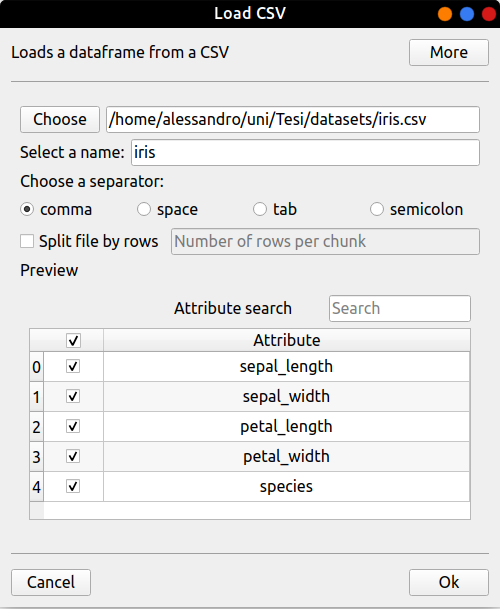
\includegraphics[width=0.56\textwidth]{load-csv}
	\caption{The widget used to load a \texttt{CSV} file}
	\label{fig:load-csv}
\end{figure}
%\begin{figure}
%	\centering
%	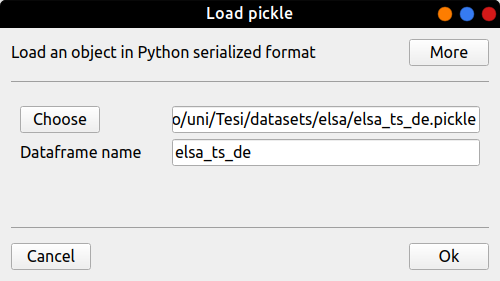
\includegraphics[width=0.7\textwidth]{load-pickle}
%	\caption{The widget used to load a Pandas dataframe with \texttt{pickle}}
%	\label{fig:load-pickle}
%\end{figure}
DataMole can import tabular datasets from \texttt{CSV} and \texttt{pickle} files that contain serialised Pandas dataframes. Notice that \texttt{pickle} files may contain any Python object, but only Pandas dataframes can be loaded in DataMole.\\
By clicking \lstinline[language=bash]|File > Import > "From csv"|, the editor shown in \cref{fig:load-csv} appears. It allows to choose the file separator and to select which columns to load. Columns can be selected in the provided table, that, depending on the size of the dataset, may require some time to be shown. Big datasets can be loaded in multiple dataframes, by selecting \textit{"Split file by rows"} and specifying the maximum number of rows per dataframe. Clicking the \textit{"More"} button opens a side panel with additional information on the operation.\\
Similarly, the widget to load a \texttt{pickle} dataframe can be opened clicking \lstinline[language=bash]|File > Import > "From pickle"|.\\
Every imported dataset will be visible in the \textit{workbench}, the widget that lists all loaded dataframes, visible in \cref{fig:main-window-man}.

\subsection{Exporting a dataset}
\begin{figure}
	\centering
	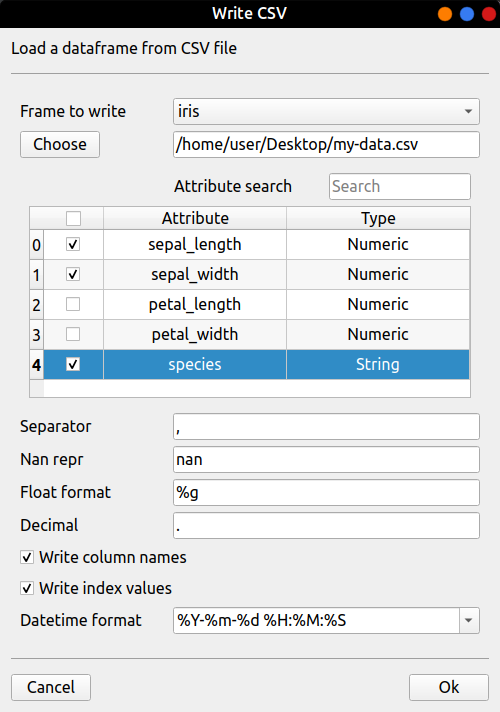
\includegraphics[width=0.56\textwidth]{save-csv}
	\caption{The widget used to export a dataframe in \texttt{CSV} file}
	\label{fig:save-csv}
\end{figure}
Loaded dataframes can be exported in \texttt{CSV} or \texttt{pickle} files. The latter option is useful to continue working on the dataset outside of DataMole, because every Python script can be used to load these files.\\
\cref{fig:save-csv} shows the widget for \texttt{CSV} export. DataMole can load multiple dataframes, thus it is required to select which one to export using a combo box. Clicking on \textit{"Choose"} opens a dialog window for selecting the save path location. The attributes to be included can be selected in the table, and many common options can be set. 

\subsubsection{Applying operations}
\begin{figure}
	\centering
	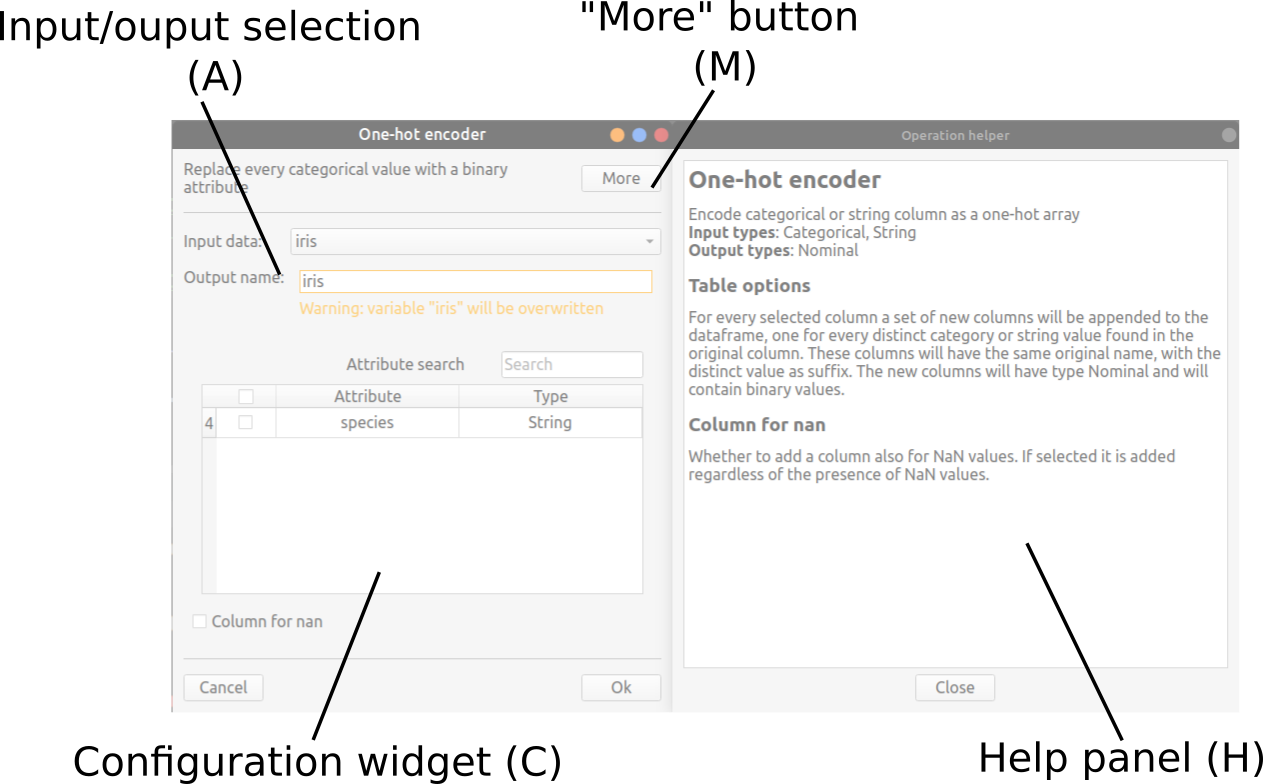
\includegraphics[width=0.85\textwidth]{editor-widget}
	\caption{The \textit{editor widget} used to configure the one-hot encoder and its help window}
	\label{fig:editor-widget-single-man}
\end{figure}
When an operation is selected in (A) and the \textit{"Apply"} button is pressed, the operation \textit{editor widget} is opened, like the one shown in \cref{fig:editor-widget-single-man}, used to one-hot encode columns. Every editor has an header with a brief description of the operation and a \textit{"More"} button on the right (M). By clicking on it, an help window with information on the operation and on the required parameters will be opened (H).\\
Below the header, a combo box allows to select the dataset to transform and a text box can be used to insert the name of the output dataset (A). After the options are confirmed with the \textit{"Ok"} button the operation will be applied and its result will be written in a \textit{workbench} variable with the specified output name. The output name defaults to the input name, thus the transformed dataset will replace the original one if the name is not edited.\\ Depending on the operation many options may need to be configured in (C). In the example the operation only requires to select the columns to encode and whether or not NaN values should be considered.\\

\subsection{The Attribute panel}\label{ssec:att-panel-man}
\begin{figure}
	\centering
	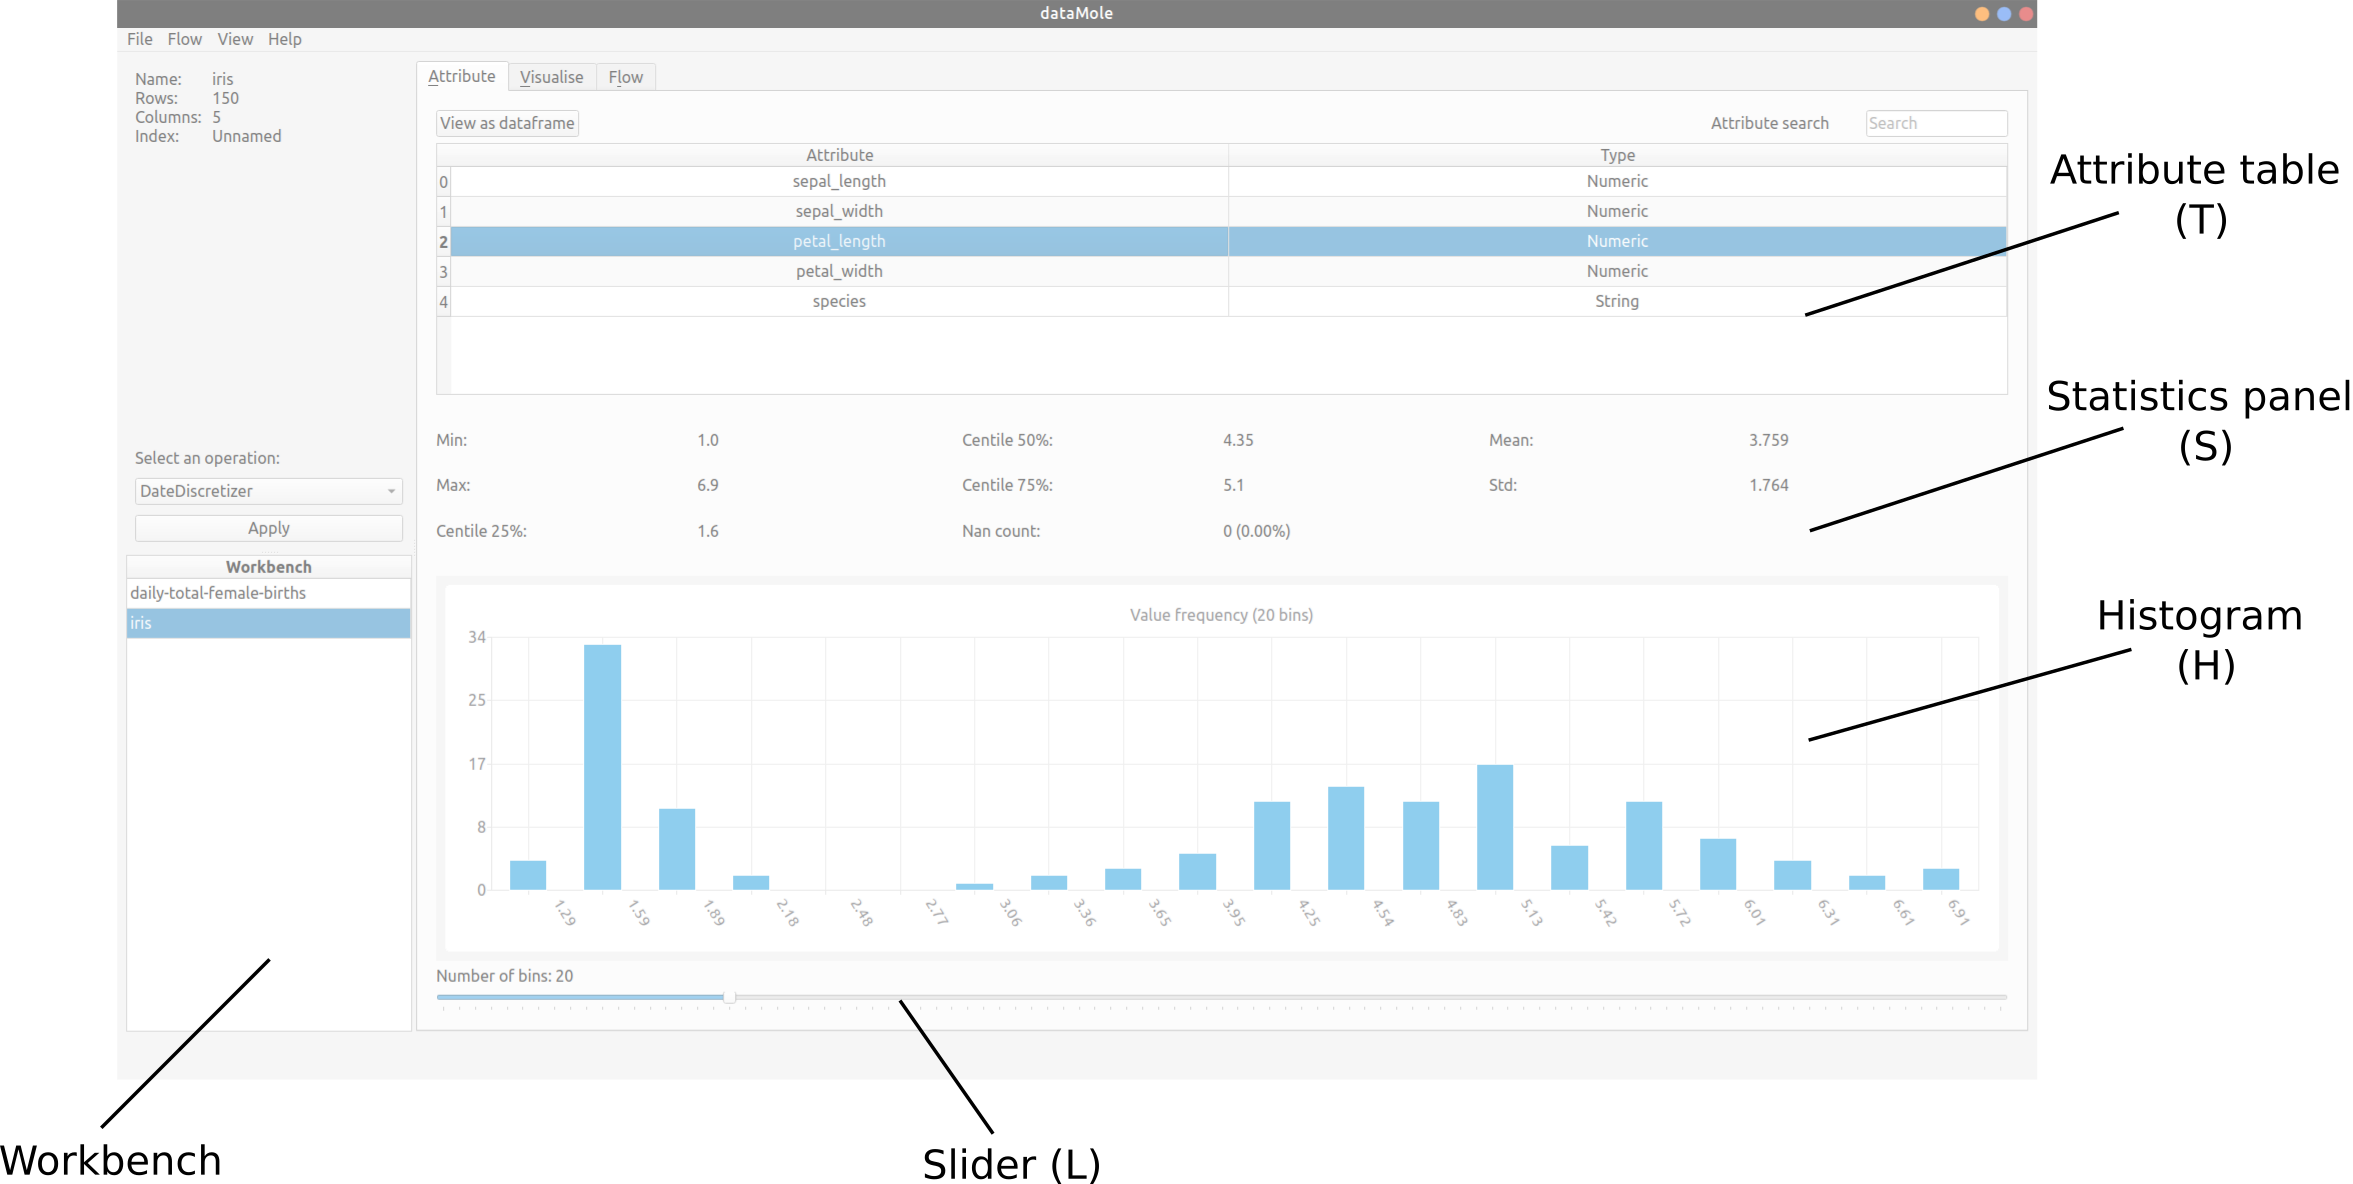
\includegraphics[width=\textwidth]{attribute-panel}
	\caption{The main window set on the \textit{Attribute panel}}
	\label{fig:attribute-panel}
\end{figure}
This panel is displayed on the left side of \cref{fig:attribute-panel}, positioned inside the tabbed widget. It provides some basic features to get an overview of the content of a dataset.\\
The \textit{attribute table} (T) displays the column names and their types: every row represents a column (i.e. an attribute) of the dataset. Column names can be changed by double clicking the cell and typing in the new name. All column names should be unique, so duplicated names will be rejected. \\
Above the table a search bar allows to search through attributes. Search by regular expression is also supported using Perl-style syntax. The search is case-insensitive.\\
The \textit{statistics panel} (S) and the \textit{histogram} (H) show information about the currently selected column, that can be changed by clicking on a row of table (T). The histogram shows the number of occurrences of every distinct values for \textit{string} and \textit{categorical} attributes, while \textit{numeric} or \textit{datetime} are first discretized in a predefined number of equal-sized intervals. This number can be changed by moving the slider below the chart (L).

\subsection{The View panel}\label{ssec:view-panel-man}
This tab groups DataMole visualisation features. Currently it supports the creation of a scatterplot matrix, to inspect feature correlation, and a line chart to plot time series.

\subsubsection{Scatterplot matrix}
\begin{figure}
	\centering
	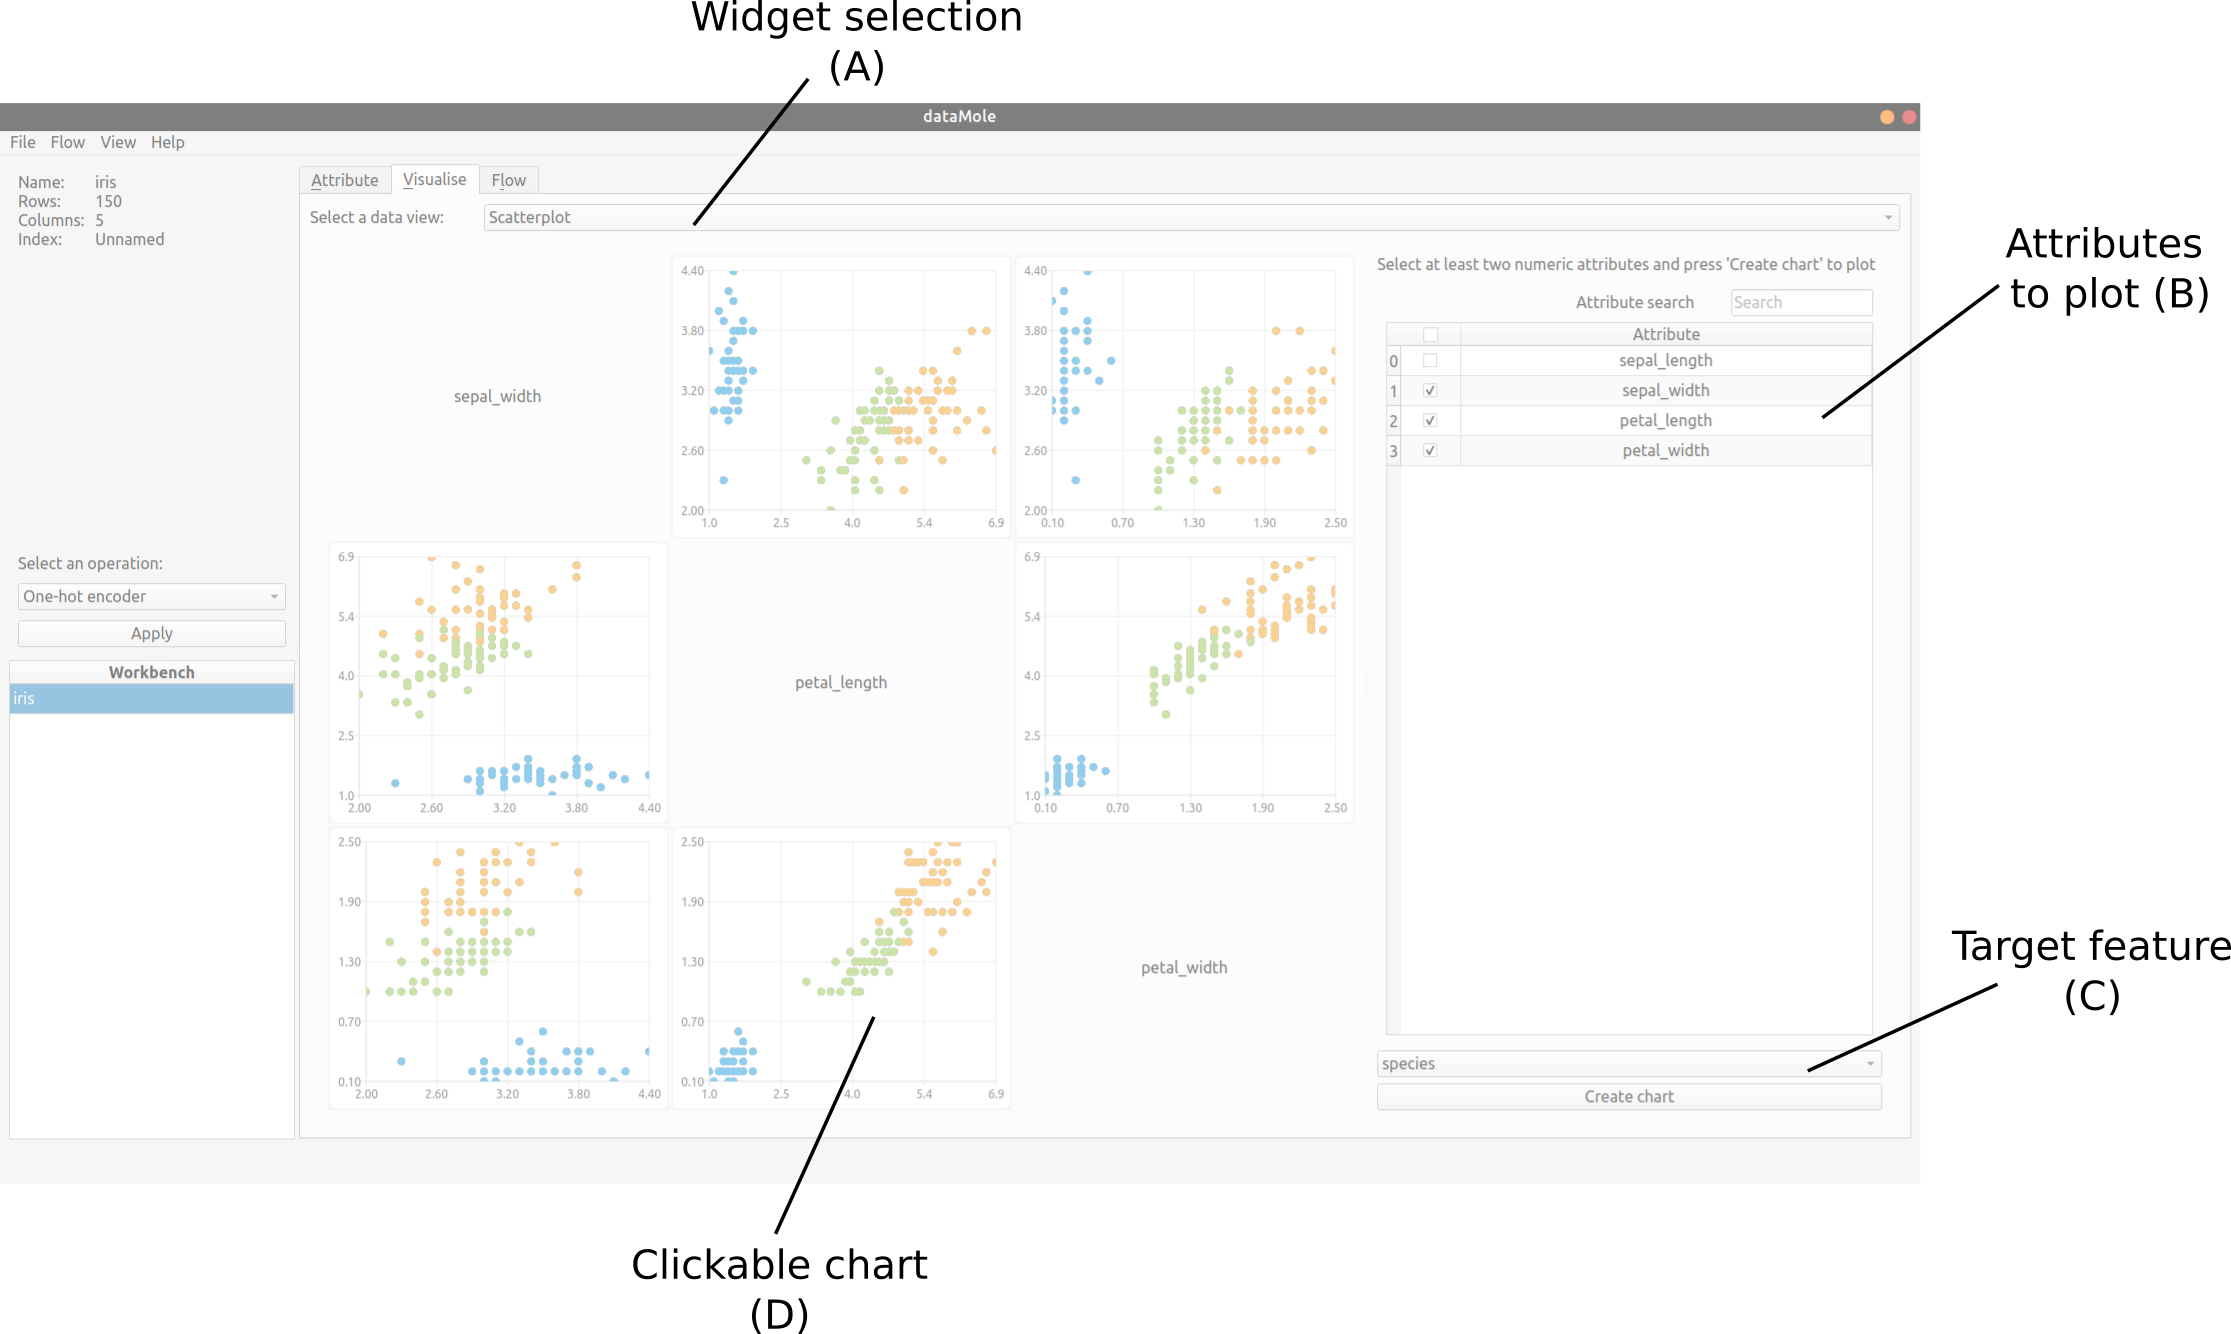
\includegraphics[width=\textwidth]{scatterplot-matrix}
	\caption{A scatterplot matrix with 3 attributes}
	\label{fig:scatterplot-matrix}
\end{figure}
\begin{figure}
	\centering
	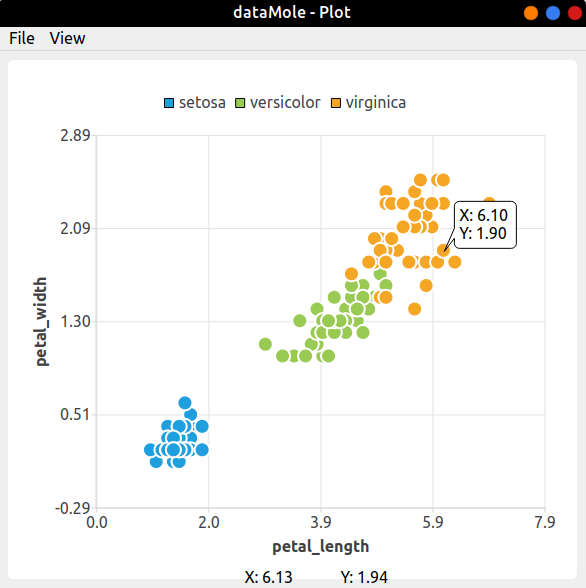
\includegraphics[width=0.6\textwidth]{scatterplot}
	\caption{A scatterplot displayed in a new window}
	\label{fig:scatterplot-single}
\end{figure}
A scatterplot matrix with 3 attributes is shown in \cref{fig:scatterplot-matrix}. A dataset must be selected in the \textit{workbench} and the attributes to plot can be chosen in widget (B). Scatterplot dots are usually coloured differently depending on the values of a target attribute, that can be chosen using the combo box below the table (C).\\
Double clicking a scatterplot opens it in a new window, like in \cref{fig:scatterplot-single}. Here dots can be hovered to inspect their values and the chart can be zoomed and stretched as required. The content of the window can additionally be saved as an image in different formats (\texttt{PNG}, \texttt{JPEG}, \texttt{BMP}, \texttt{XMP}).\\
The combo box in (A) allows switching between the two chart types.

\subsubsection{Time series plot}
\begin{figure}
	\centering
	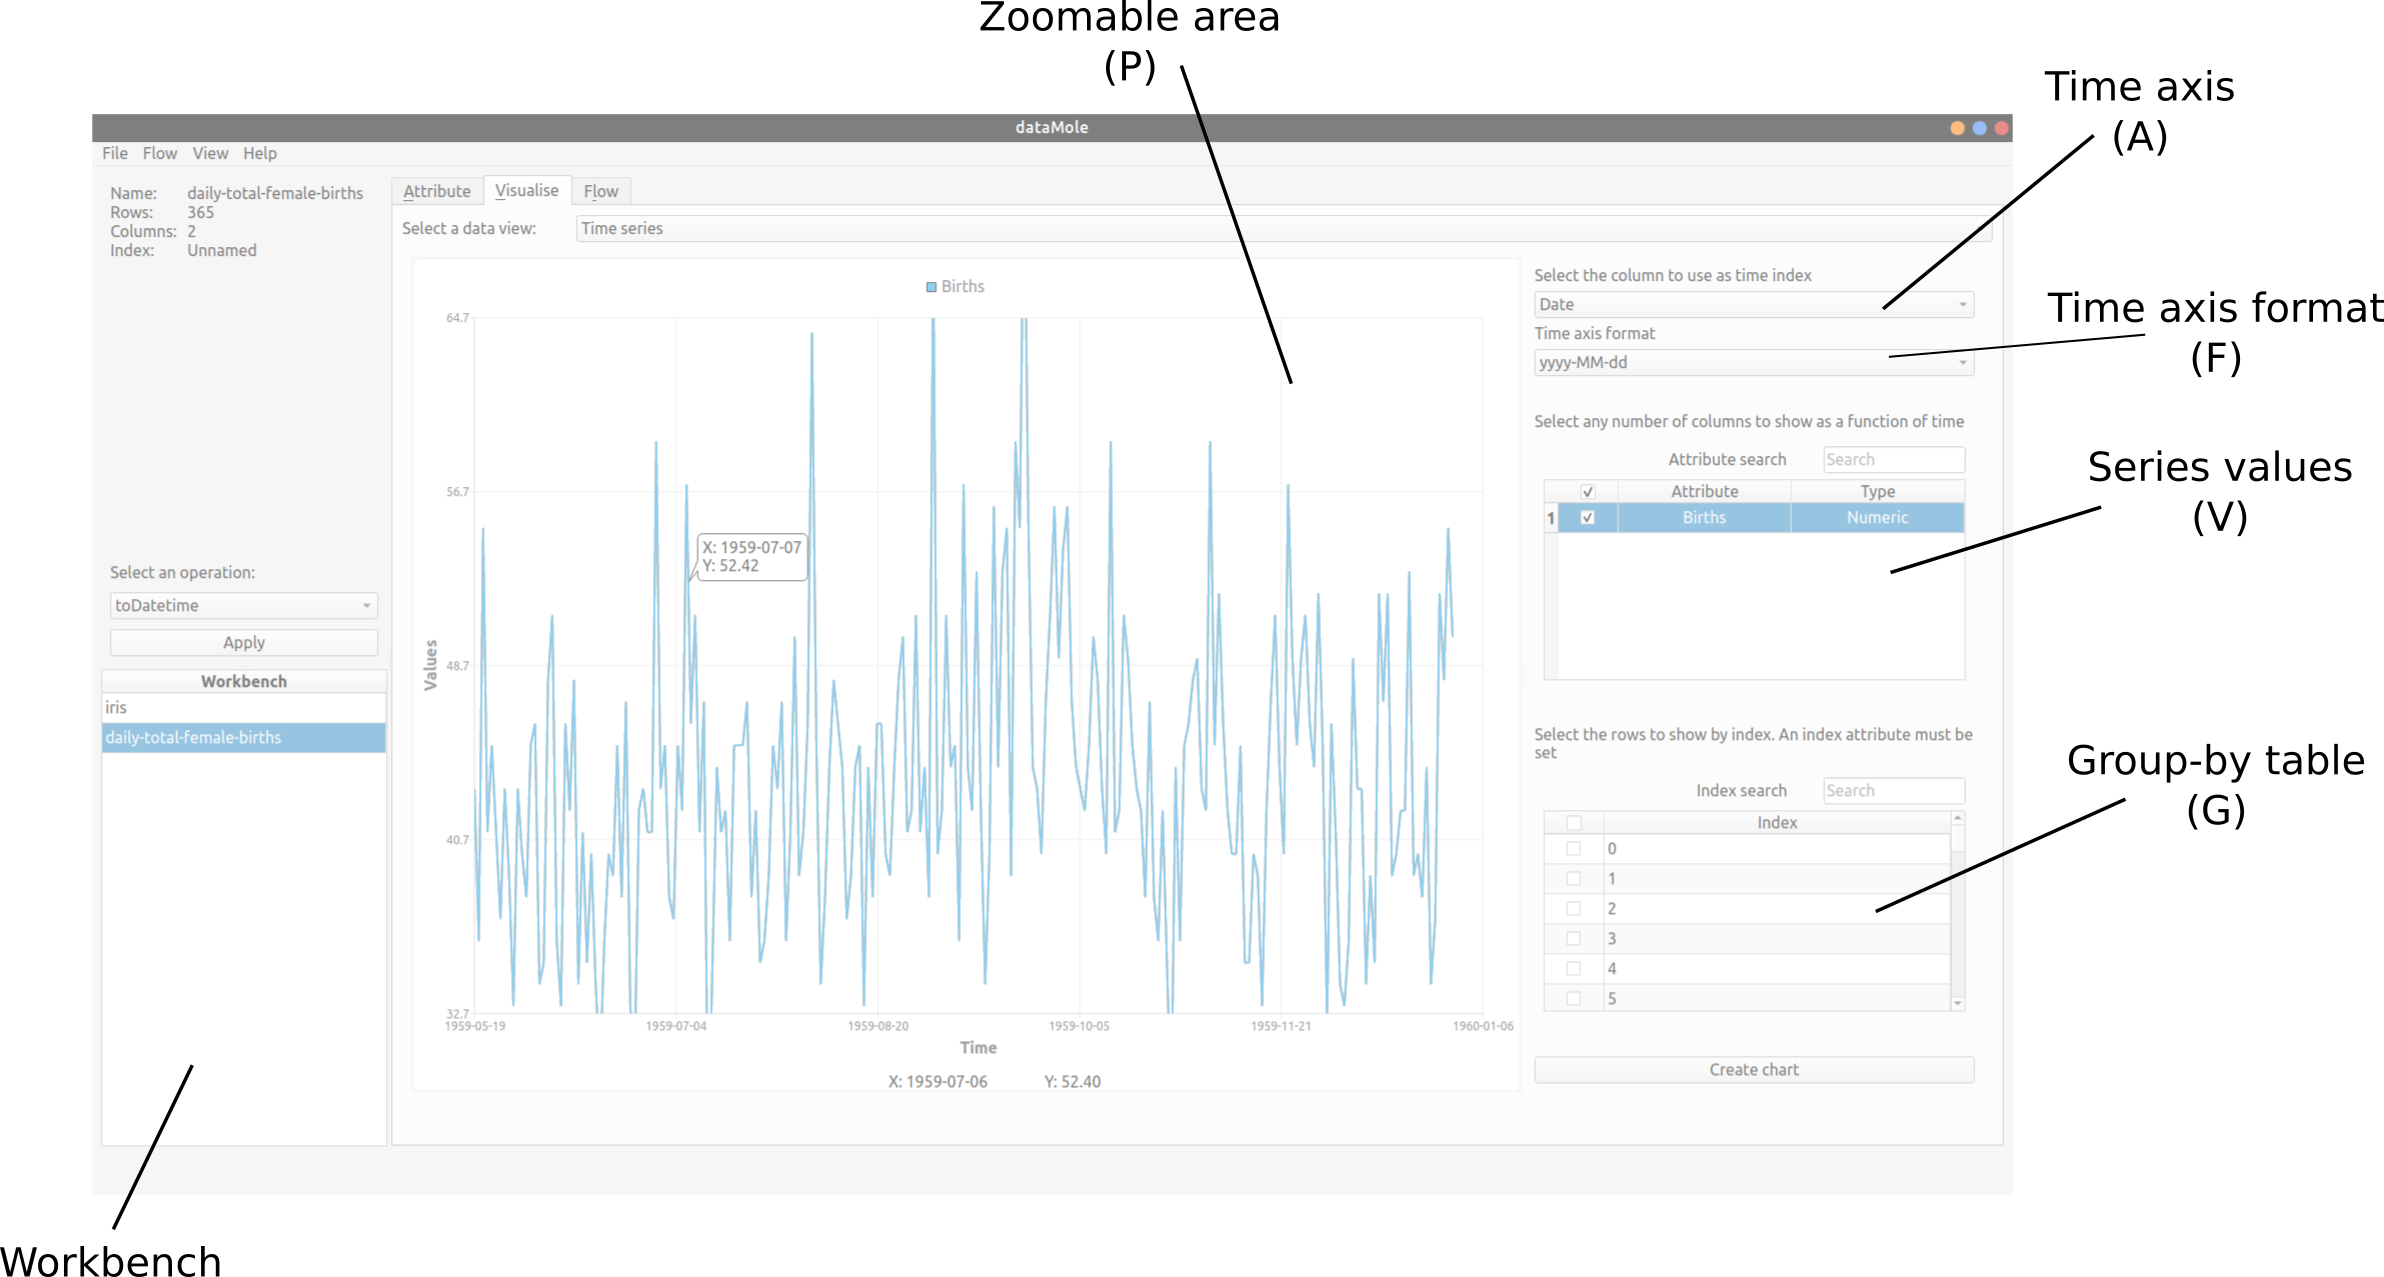
\includegraphics[width=\textwidth]{time-series-births}
	\caption{A time series displayed with a line chart}
	\label{fig:time-series-births}
\end{figure}
Time series can be represented in a line chart like in \cref{fig:time-series-births} using this widget. First, the dataset must be selected in the \textit{workbench}. Then the attribute that contain the time axis labels must be selected in (A): it must be either an attribute with type \textit{datetime} or with \textit{ordinal} type, since a order must be defined between its values. If a \textit{datetime} attribute is selected the label format for visualisation in the horizontal axis can be changed in (F).\\ 
The time dependent attributes can then be selected in table (V). The chart area (P) is interactive and can be zoomed and moved around. The initial state of the chart can be restored by using the \lstinline[language=bash]|Ctrl+R| shortcut.\\
If an index is set in the dataframe, table (G) can be used to select a subset of indices to plotted. When the chart is created, data are grouped by index, and every group is considered a different time series to plot. This feature was included in order to plot time series which have been extracted by longitudinal datasets. The documentation of the \textit{Time series extraction} operation provides more details about this.

\subsection{The Flow panel}\label{ssec:flow-panel-man}
\begin{figure}
	\centering
	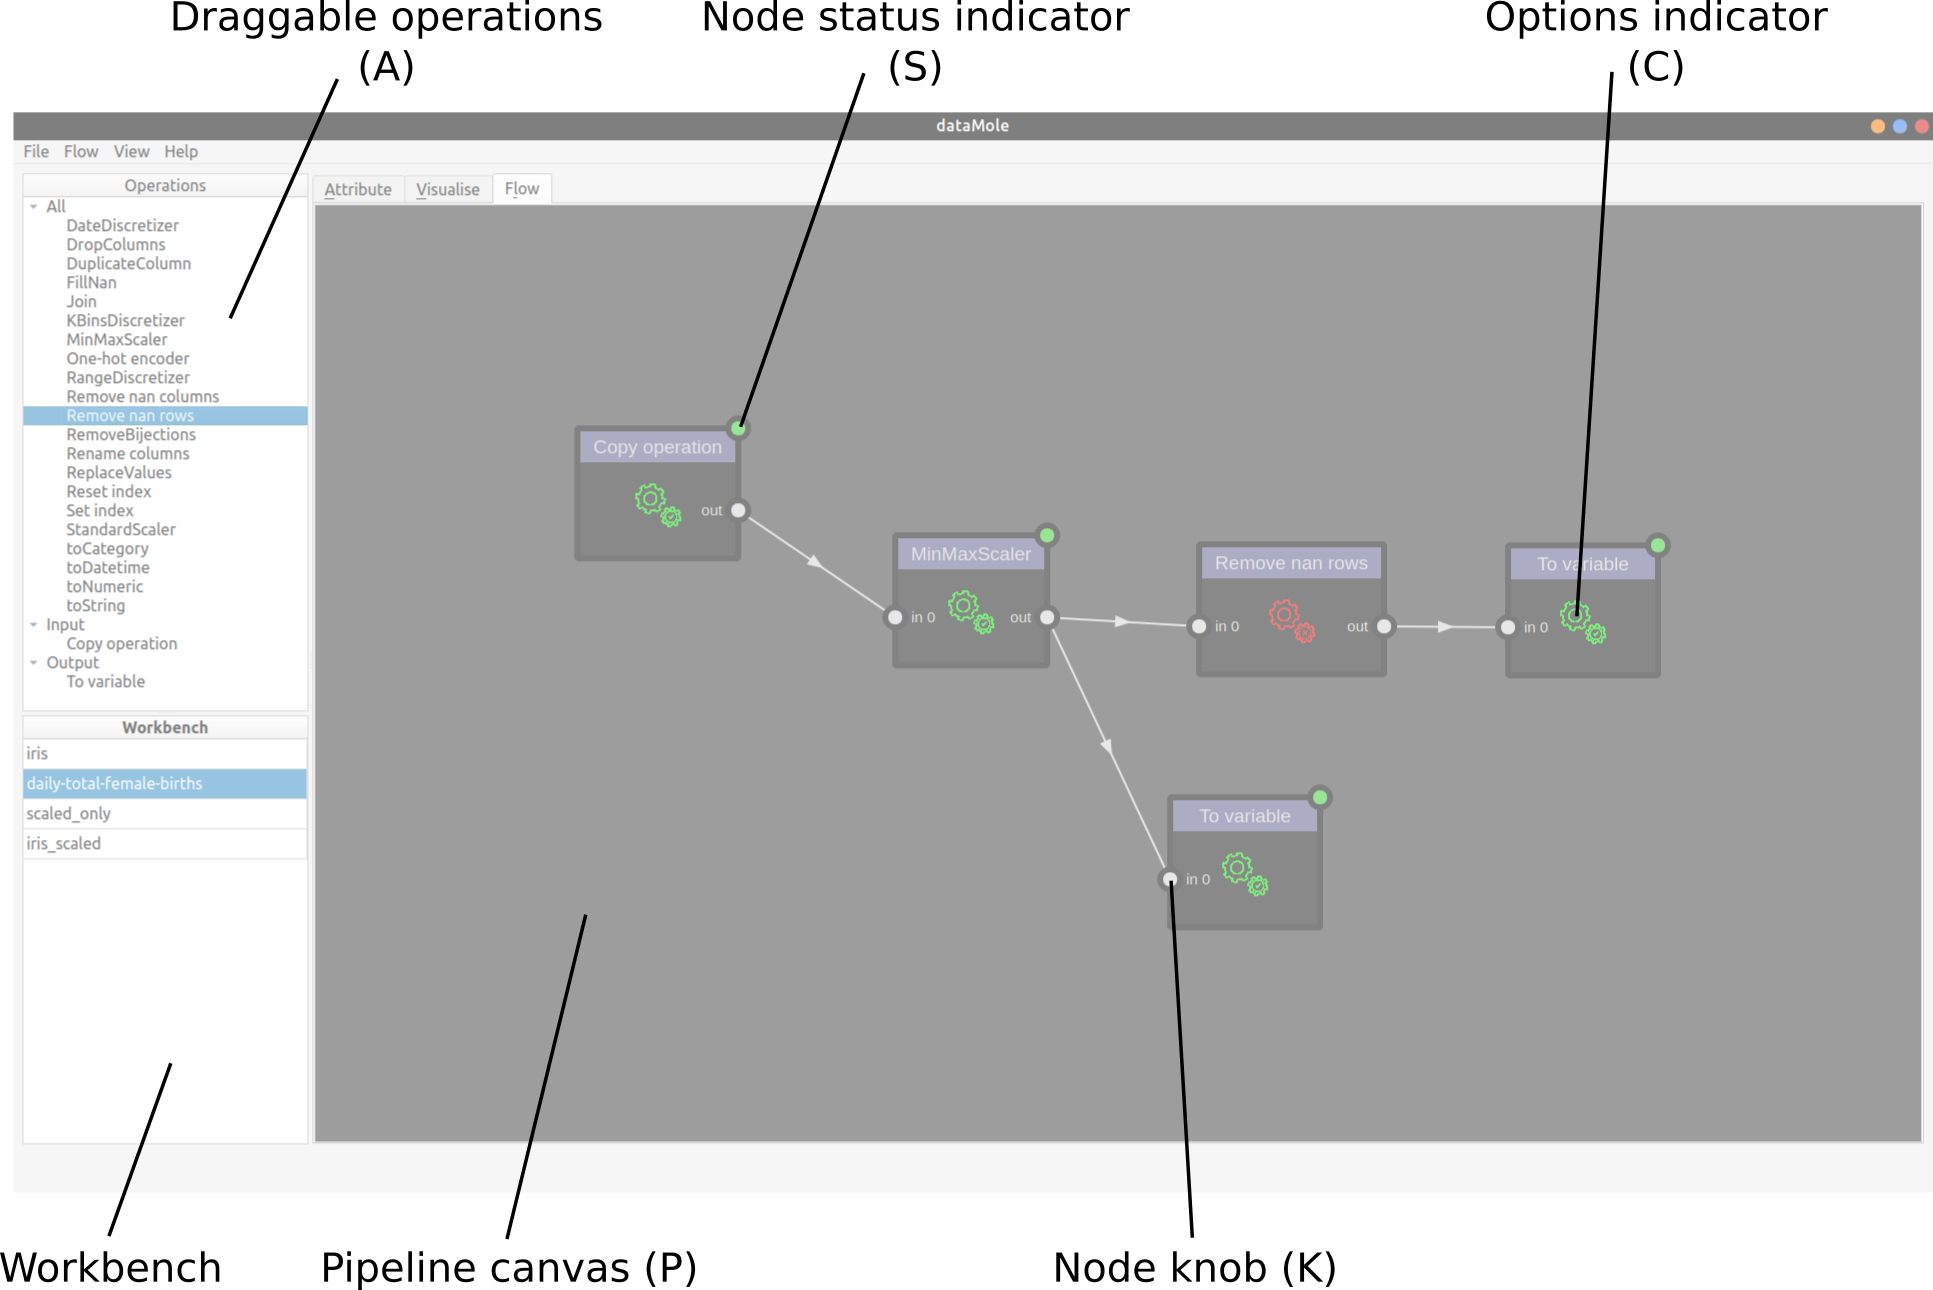
\includegraphics[width=\textwidth]{flow-panel}
	\caption{A simple pipeline defined in the \textit{Flow panel}}
	\label{fig:flow-pipeline}
\end{figure}
The last available panel provides an alternative approach to dataset transformation: the same operations that could be applied singularly from both the \textit{Attribute} and \textit{View panel} can be chained together to form a pipeline where the output of a node becomes the input of its successors. \cref{fig:flow-pipeline} displays a pipeline composed of 5 steps.\\
Steps can be added to the pipeline canvas (P) by dragging them from the list of operations on the left side of the window (A). Every step is represented graphically with a node that has some \textit{knobs} (K) on the left an right side. Nodes can be connected by clicking a \textit{knob} on the source node and dragging the interactive edge up to the target node, where it must be dropped. Most operations require some parameters before the pipeline can be executed. In order to do this every operation has a \textit{widget editor} that is used to configure them. For instance the widget shown in \cref{fig:flow-editor-sample} is the editor widget for the min-max scaler operation. These editors can be opened by double clicking the operation nodes in the pipeline, and when options are set they can be confirmed with the \textit{"Ok"} button. At this point the operation is configured an its \textit{options indicator} (C) turns green.\\
The pipeline canvas can be zoomed and moved around using the mouse wheel. Pressing the \lstinline[language=bash]|F| key while the canvas is focused fits the view to its content.\\
When the pipeline has been configured it can be executed by clicking \lstinline[language=bash]|Flow > Execute|. Once started, a \textit{status indicator} appears above every node (S). It is grey for nodes that must still be executed, green for completed nodes, yellow for running nodes and red for nodes that failed with an error. This status can be reset by clicking \lstinline[language=bash]|Flow > "Reset status"|.\\
Pipelines can also be imported and exported using the respective entries in the menu bar: \lstinline[language=bash]|Flow > "Load"| and \lstinline[language=bash]|Flow > "Save"|.
\begin{figure}[p]
	\centering
	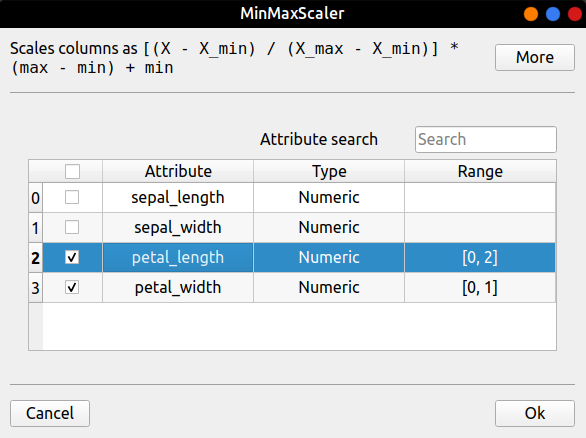
\includegraphics[width=0.8\textwidth]{scale-editor-w}
	\caption{The \textit{editor widget} for the operation used to scale columns}
	\label{fig:flow-editor-sample}
\end{figure}
\begin{figure}[p]
	\centering
	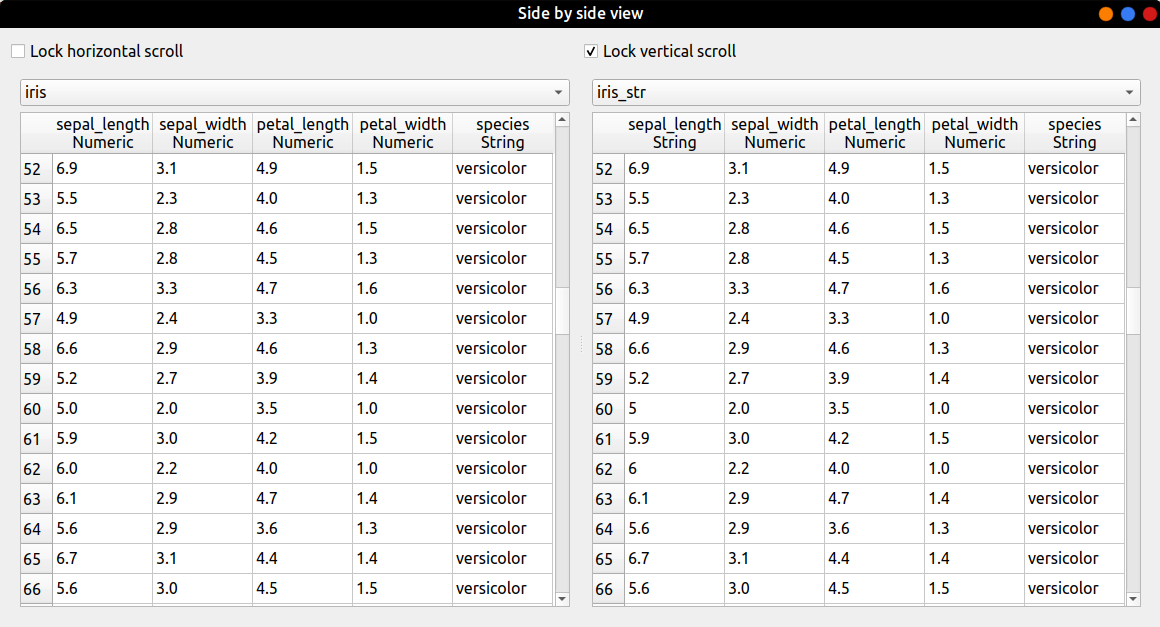
\includegraphics[width=\textwidth]{compare-df}
	\caption{Comparison of two dataframes side by side}
	\label{fig:compare-df}
\end{figure}

%\clearpage
\subsection{Other features}
\subsubsection{Dataframe visualisation}
Menu entry \lstinline[language=bash]|View > "Compare dataframes"| opens a window where two dataframes can be selected and compared side by side, like in \cref{fig:compare-df}.
It is also possible to visualise single dataframes in a similar table, by clicking button "View as dataframe" in the \textit{Attribute panel}.\\
These views are read-only, thus datasets can not be edited from within DataMole.

\subsubsection{Logging facilities}
Whenever a pipeline is executed from the \textit{Flow panel} DataMole writes an execution report inside the \texttt{logs/graph} folder. Every log file is named with the timestamp of when it was created and includes information on the configuration of every operation (like user supplied options) and eventual parameters computed during execution. Also operations applied singularly from the \textit{Attribute panel} are logged in the same way inside the \texttt{logs/ops} folder. In this case every program session initialises a new log file.\\
Additionally debug information as well as critical errors are logged inside \texttt{logs/app}. These logs can be useful to debug software crashes and unexpected behaviours.\\
The log directory can be opened using the predefined window manager from menu 
\lstinline[language=bash]|Help > "Open log directory"|. \\
Finally, option \lstinline[language=bash]|Help > "Delete old logs"| clean the log directory removing all but the 5 most recent files.

\subsection{Extraction of a time series: an example}\label{ssec:ts-extract}
\begin{table}[!ht]
	\centering
	{\renewcommand{\arraystretch}{1.2}
		\rowcolors{2}{white}{tableCol}
		\begin{tabular}{cc}
			\rowcolor{tableHead}
			\color{white}\textbf{Date} & \color{white}\textbf{Births} \\
			1959-01-01 & 35 \\
			1959-01-02 & 32 \\
			1959-01-03 & 30 \\
			\vdots & \vdots \\
			1959-12-30 & 55\\
			1959-12-31 & 50
		\end{tabular}
	}
	\caption{Some rows from the \textit{daily-total-female-births} dataset}
	\label{tab:female-births-str}
\end{table}
\begin{table}[!ht]
	\centering
	{\renewcommand{\arraystretch}{1.2}
		\rowcolors{2}{white}{tableCol}
		\begin{tabular}{cccc}
			\rowcolor{tableHead}
			\color{white}\textbf{idauniq} & \color{white}\textbf{wpwlyy} & \color{white}\textbf{wpbima} & \color{white}\ldots \\
			121321 & \ldots & \ldots &\\
			121323 & \ldots & \ldots &\\
			121332 & \ldots & \ldots &\\
			\vdots & & &
		\end{tabular}
	}
	\caption{Structure of a wave of the ELSA dataset}
	\label{tab:elsa-wave-str}
\end{table}
The dataset used to plot the time series in \cref{fig:time-series-births} is composed of 365 entries, each with a date (under column \textit{Date}) and the number of female births on that day (column \textit{Births}). A sample of this dataset is reported in \cref{tab:female-births-str}.
The \textit{View panel} can understand dataset in this simple format: it is only necessary to convert the \textit{Date} attribute to \textit{datetime}, set it as the time axis and select the time-dependent attributes, which is only \textit{Births} in this example.\\
Longitudinal dataset like ELSA or HRS are not so simple: first there is no attribute representative of the time axis, but rather this information is implicitly conveyed by putting the variables from different waves in distinct files, or, if they are all in the same file, by renaming the variables to reference the wave they belong to (e.g. \textit{varA\_wave1}, \textit{varA\_wave2}, etc.). Hence, with these datasets the temporal information must be made explicit, by defining a time axis and, with the user help, link every column of the datasets to their point in this axis. For instance the file containing ELSA data from wave 3 has the structure described in \cref{tab:elsa-wave-str}. For the purpose of this example, only 3 attributes are listed: the \textit{idauniq} attribute contains the unique cross-wave identifier, \textit{wpwlyy} is the amount of gross income gained from the respondent work at the end of the previous year and \textit{wpbima} is the average monthly income from business during the previous 12 months (from the interview). Other waves follow the same scheme, even though variable names can sometimes change across different waves.
%An in-depth overview of the ELSA dataset has been covered in section \ref{sssec:elsa-over}.\\
\begin{figure}[!ht]
	\centering
	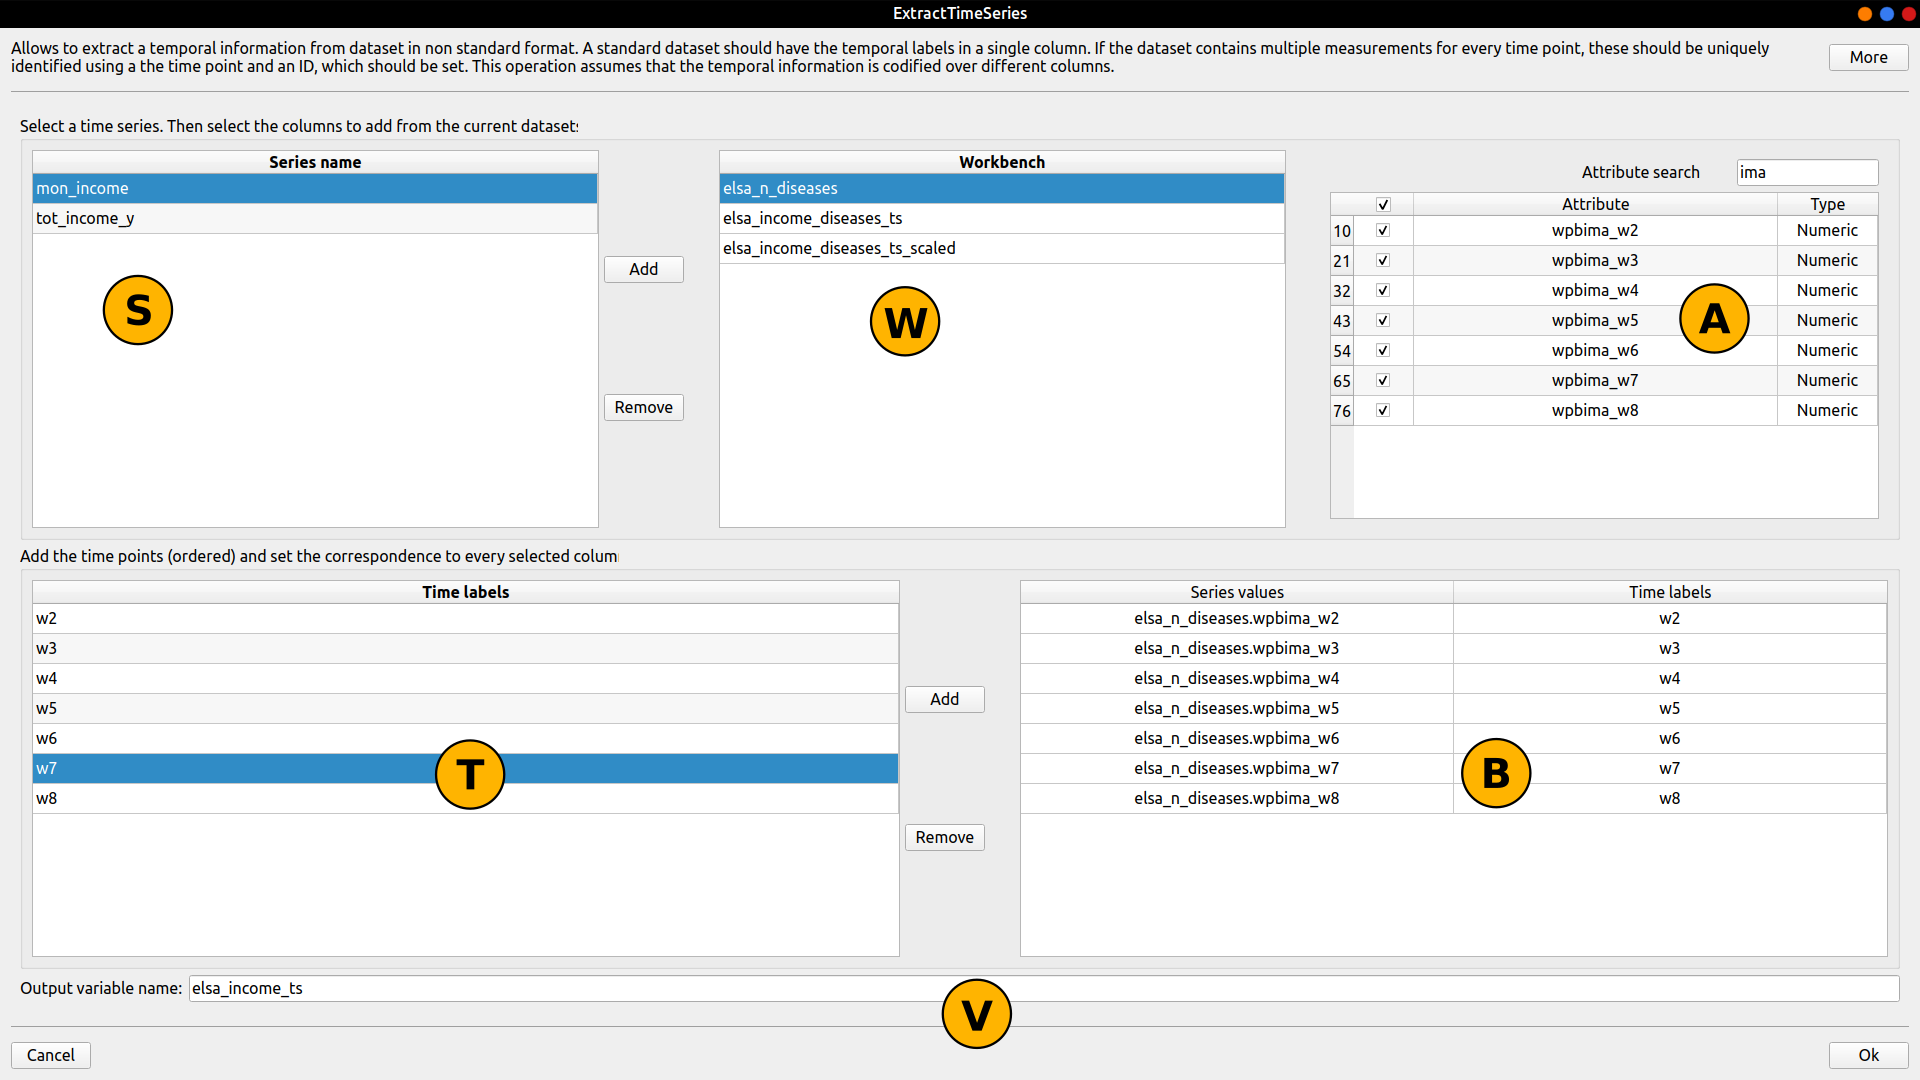
\includegraphics[width=\textwidth]{example_ts/extract_ts_s1}
	\caption{Extraction of time series from ELSA attribute \textit{wpbima}}
	\label{fig:elsa-extraction-wpb}
\end{figure}
Suppose we want to visualise how the respondent income changes from wave 2 to 8 and plot it as a time series: there is no immediate way to do it, and we have to manipulate this dataset and transform it into a time series that can be identified and used in the \textit{View panel}. The \textit{time series extraction} operation is designed for this use case. \cref{fig:elsa-extraction-wpb} shows the widget used to configure the operation. In this case the relevant attributes (\textit{wpbima} and \textit{wpwlyy}) were previously extracted from their files and merged together in a single dataframe using the \textit{join} operation. They were also renamed by appending the name of the waves they referred to (\textit{\_w2} for the second wave, \textit{\_w3} for the third and so on). This attributes contain a majority of NaN values: for the purpose of this example, they were filled with the per-column average, even though, in a real use case, they would probably be unusable.\\
In \cref{fig:elsa-extraction-wpb} two time series are defined and added to list \textit{(S)}: \textit{mon\_income} for attribute \textit{wpbima}, and  \textit{tot\_income\_y} for \textit{wpwlyy}.\\
Then every time series is populated with its values: since we are interested in the average monthly income from the second to the eight wave, attributes from \textit{wpbima\_w2} to \textit{wpbima\_w8} are selected in table \textit{(A)}. Here all attributes are taken from a single dataframe, but it is generally possible to select attributes from different dataframes by choosing the right ones in the workbench shown in section \textit{(W)}.\\
The next step is the association of these attributes to a time point (the wave in this case). Thus, after defining an appropriate number of labels for the time axis in the bottom-left table \textit{(T)}, we associate every relevant column to its time label in the bottom-right table \textit{(B)}: here we are basically telling DataMole that \textit{wpbima\_w2} contains the values of the attribute \textit{wpbima} for wave 2, \textit{wpbima\_w3} contains the values for wave 3 and so on. Series \textit{tot\_income\_y} is built in the same way, by selecting the attributes \textit{wpwlyy} from the various waves. Finally, a name for the dataset is set in \textit{(V)} and the operation is started.\\
The result of this operation is a new dataset with the structure shown in \cref{tab:elsa-ts-extracted-str}. Every respondent is associated to 7 entries, each containing a distinct time label (\textit{time} attribute) and the values of the \textit{wpwlyy} and \textit{wpbima} columns, respectively under columns \textit{tot\_income\_y} and \textit{mon\_income}.\\ \noindent
\begin{table}
	\centering
	{\renewcommand{\arraystretch}{1.2}
		\begin{tabular}{cccc}
			\rowcolor{tableHead}
			\color{white}\textbf{idauniq} & \color{white}\textbf{time} & \color{white}\textbf{tot\_income\_y} & \color{white}\textbf{mon\_income} \\
			\rowcolor{tableCol}	 	& w2 & \ldots & \ldots \\
			\rowcolor{tableCol}		& w3 & \ldots & \ldots \\
			\rowcolor{tableCol}		& w4 & \ldots & \ldots \\
			\rowcolor{tableCol}		& w5 & \ldots & \ldots \\
			\rowcolor{tableCol}		& w6 & \ldots & \ldots \\
			\rowcolor{tableCol}		& w7 & \ldots & \ldots \\
			\rowcolor{tableCol}
			\multirow{-7}{*}{121321}& w8 & \ldots & \ldots \\
			& w2 & \ldots & \ldots \\
			& w3 & \ldots & \ldots \\
			& w4 & \ldots & \ldots \\
			& w5 & \ldots & \ldots \\
			& w6 & \ldots & \ldots \\
			& w7 & \ldots & \ldots \\
			\multirow{-7}{*}{121323}& w8 & \ldots & \ldots \\
			\rowcolor{tableCol}		& w2 & \ldots & \ldots \\
			\rowcolor{tableCol}		& w3 & \ldots & \ldots \\
			\rowcolor{tableCol}		& w4 & \ldots & \ldots \\
			\rowcolor{tableCol}		& w5 & \ldots & \ldots \\
			\rowcolor{tableCol}		& w6 & \ldots & \ldots \\
			\rowcolor{tableCol}		& w7 & \ldots & \ldots \\
			\rowcolor{tableCol}
			\multirow{-7}{*}{121332}& w8 & \ldots & \ldots \\
			\vdots					& & &
		\end{tabular}
	}
	\caption[Structure of the dataset generated with the extraction of two time series]{Structure of the dataset generated with the extraction of two time series (\textit{tot\_income\_y} and \textit{mon\_income}) from the ELSA dataset}
	\label{tab:elsa-ts-extracted-str}
\end{table}\noindent
\noindent At this point it is possible to plot these attributes: you can see how the average monthly income and the yearly income changes for a single respondent (\cref{fig:elsa-ts-1}) or you can compare the same attribute (yearly income or monthly income) from two different respondents (\cref{fig:elsa-ts-2}). In both cases the table on the bottom (named \textit{(C)} in \cref{fig:elsa-ts-1}) must be used to select the ids of the respondents to plot. This table allows to select by dataframe index, that must be set appropriately: in this example it is set on the respondent id. Additionally when an index is selected, the chart expects to find a time attribute and some time-dependent attributes to plot for every selected index, exactly like in \cref{tab:elsa-ts-extracted-str}.
Hence table \textit{(C)} should be used only to plot time series extracted with the \textit{time series extraction} operation.
\begin{figure}
	\centering
	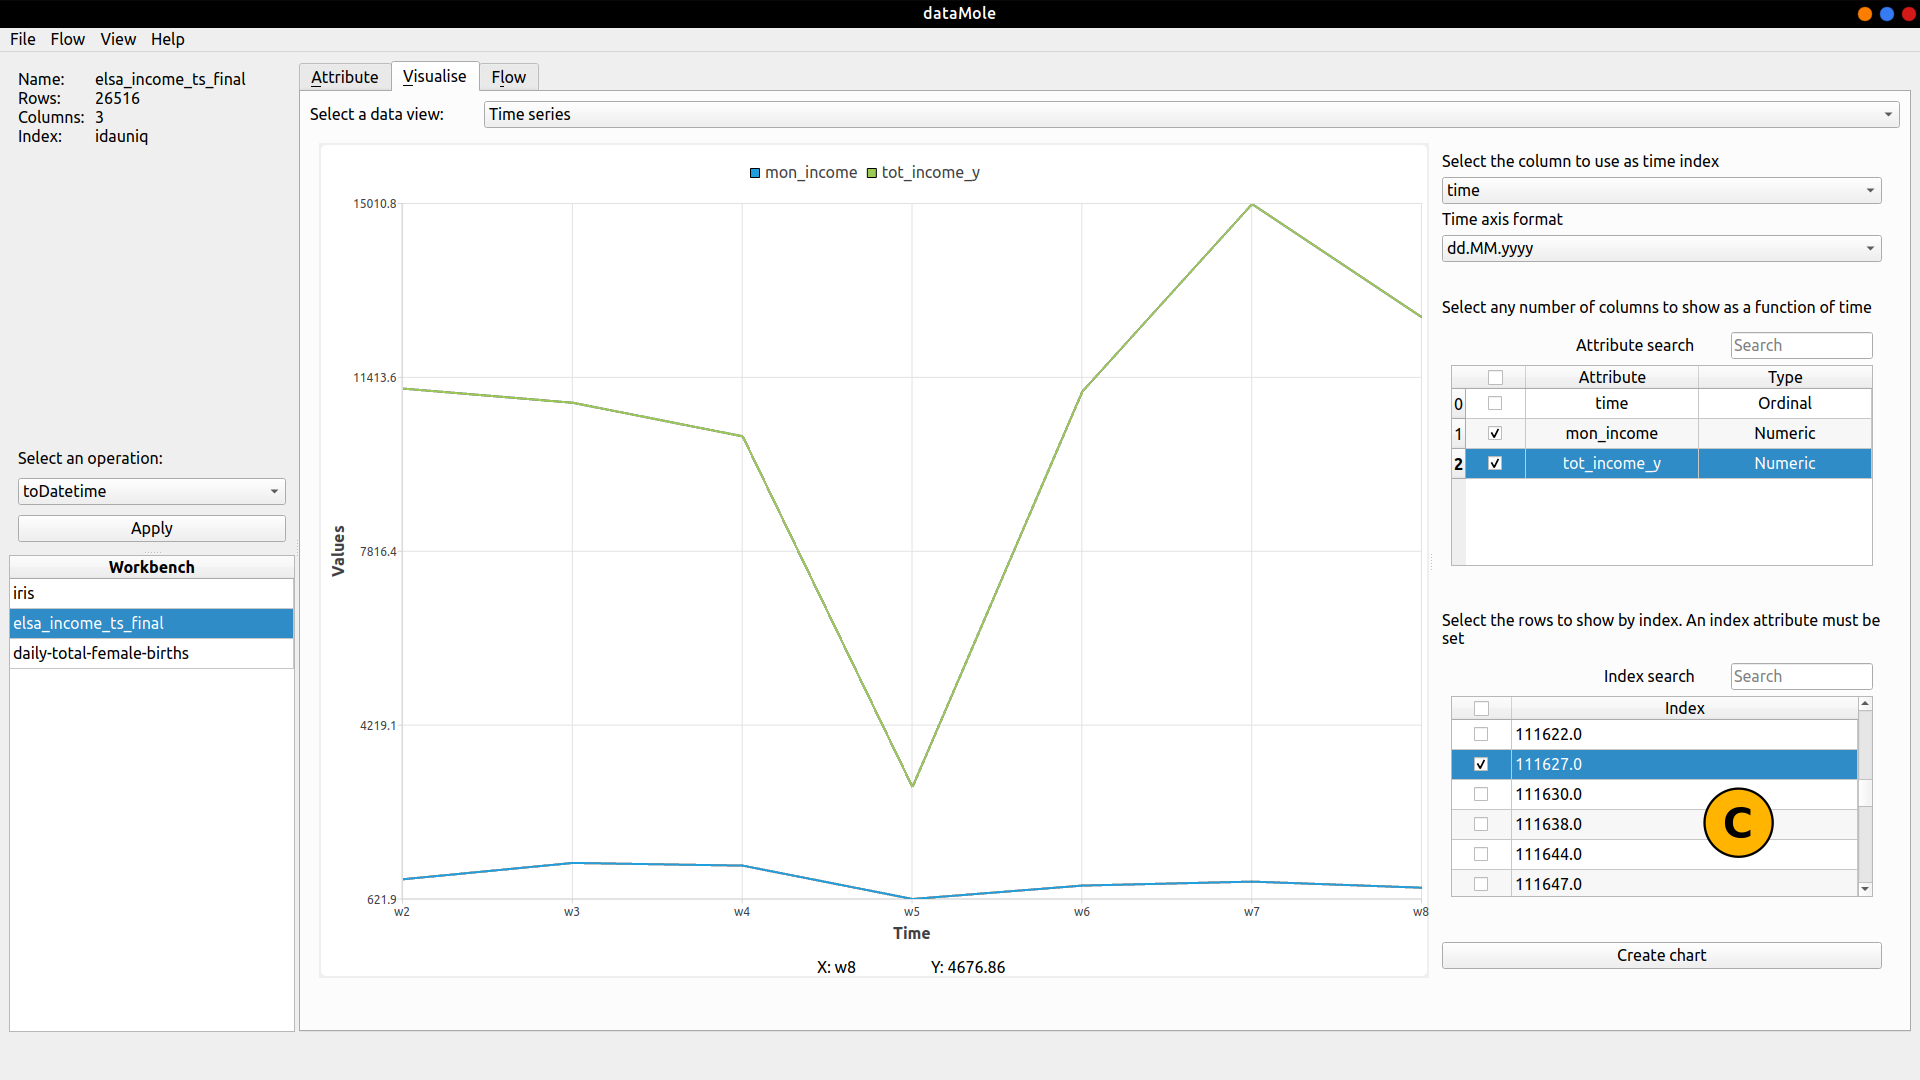
\includegraphics[width=\textwidth]{example_ts/mon_year_income}
	\caption[The average monthly income and yearly income of a single ELSA respondent measured in wave 2 to 8]{The average monthly income and yearly income of a single ELSA respondent measured in wave 2 to 8 (ELSA attributes \textit{wpbima} and \textit{wpwlyy}). The time labels for every wave are shown on the \textit{Time} axis (horizontal), while the vertical axis shows the values of the two selected attributes.}
	\label{fig:elsa-ts-1}
\end{figure}
\begin{figure}
	\centering
	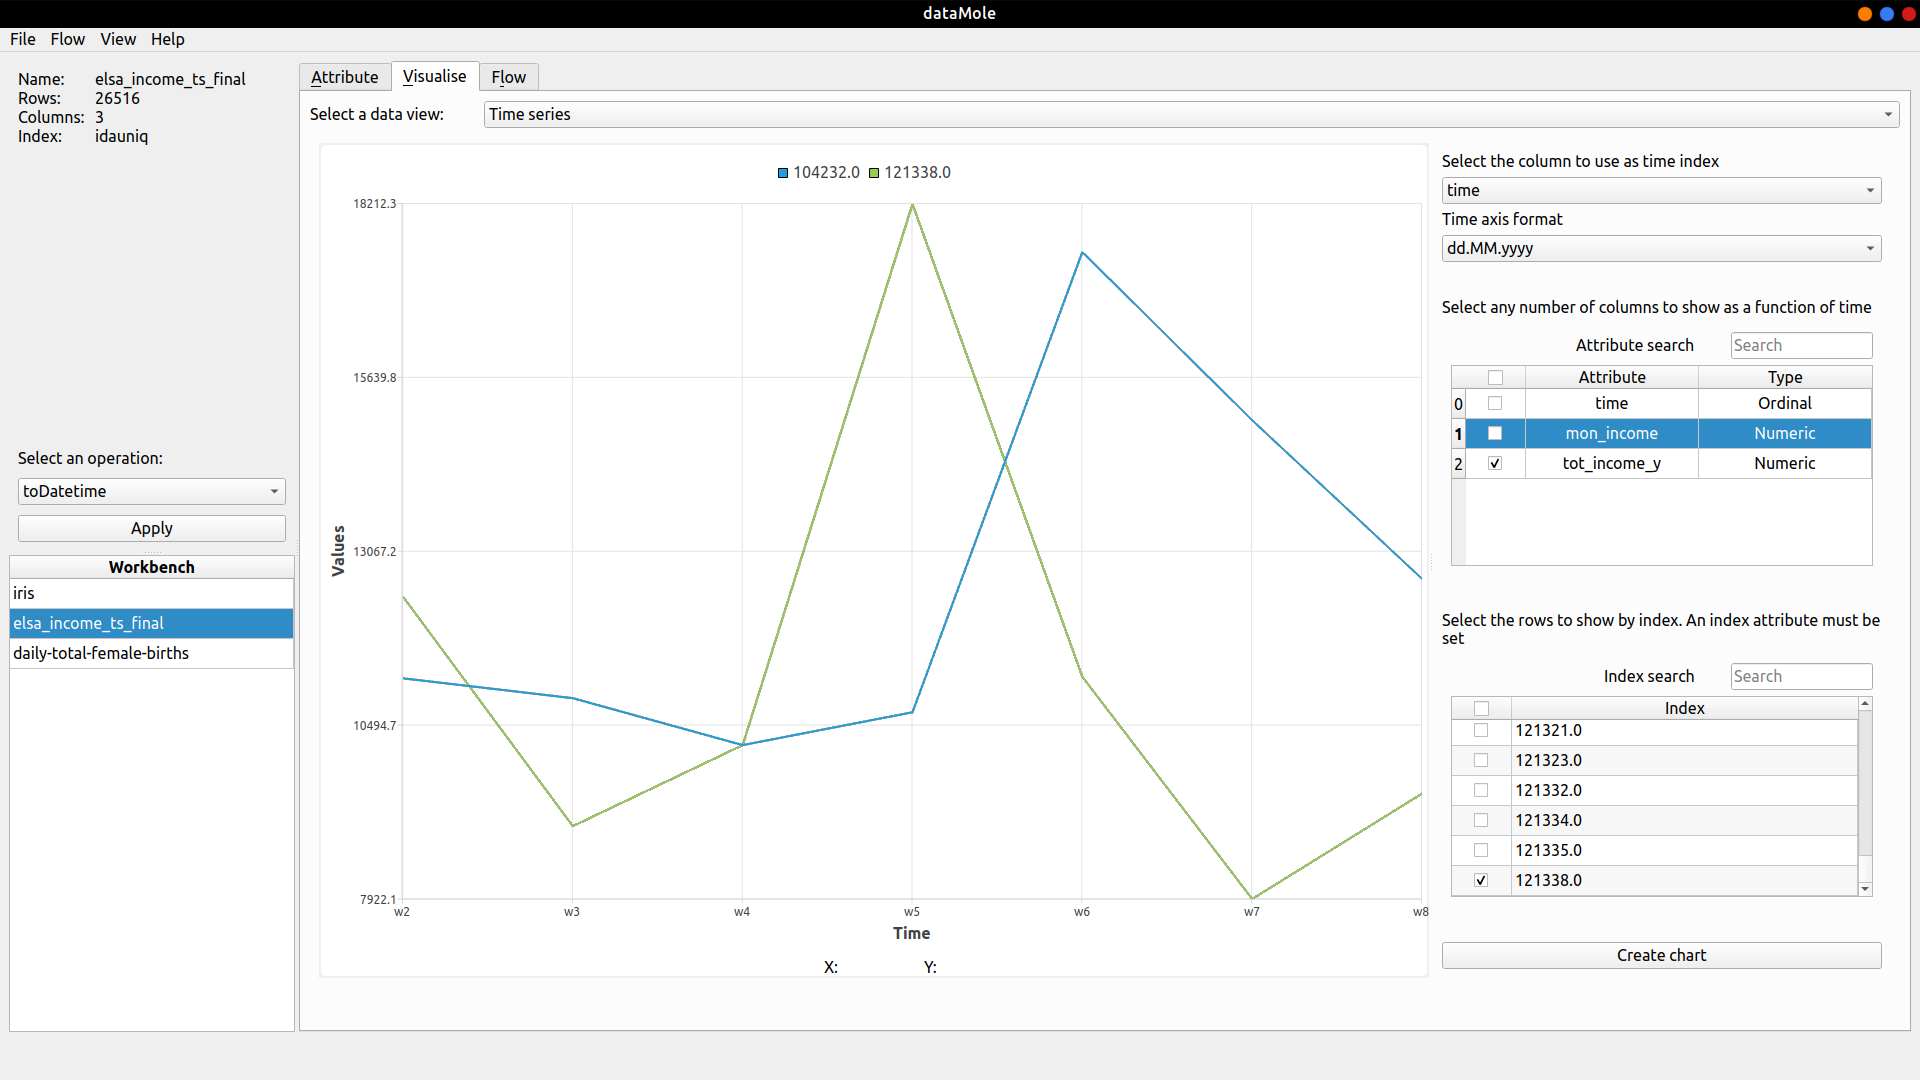
\includegraphics[width=\textwidth]{example_ts/income_y_subjects}
	\caption[The yearly income of two ELSA respondents from wave 2 to 8]{The yearly income of two ELSA respondents from wave 2 to 8 (ELSA attribute \textit{wpwlyy})}
	\label{fig:elsa-ts-2}
\end{figure}

%\backmatter
% !TEX encoding = UTF-8
% !TEX TS-program = pdflatex
% !TEX root = ../tesi.tex

%**************************************************************
% Bibliografia
%**************************************************************

%\cleardoublepage
%\chapter{Bibliography}
%
%\defbibfilter{papers}{
%	type=article or
%	type=book or
%	type=online
%}

%\raggedright
\sloppy % spezza url troppo lunghi giustificandoli

%\nocite{*}
% Stampa i riferimenti bibliografici
%\printbibliography[heading=subbibliography,title={References},filter=papers]
%
%% Stampa i siti web consultati
%\printbibliography[heading=subbibliography,title={Online resources},type=customa]

\printbibliography

% Biblio del confronto
% \printbibliography[heading=subbibliography,title={Siti web consultati per il confronto},type=customa]


\end{document}
